\documentclass[UTF8,no-math,12pt,openany,table,dvipsnames,svgnames]{book}
\usepackage{indentfirst}
\usepackage{ctex,amsmath,amssymb,mathrsfs}
\usepackage[centering,
           top=2.54cm,bottom=2.54cm,right=2.9cm,left=2.9cm,
           headsep=25pt,headheight=20pt]{geometry}
\setmainfont{Times New Roman}
\usepackage{tikz}
\usepackage{metalogo}
\usepackage{tcolorbox}
\tcbuselibrary{listings,breakable}
\tcbset{boxrule=0pt,sharp corners}
\usepackage{titlesec}
\titleformat{\chapter}{\centering\huge\bfseries}{第 \thechapter 章}{1em}{}
\usepackage[hyperindex]{hyperref}
\hypersetup{bookmarksopen=true,bookmarksopenlevel=1,bookmarksnumbered=true,
  pdftitle={tkz-euclide绘图},pdfauthor={向禹},linktoc=page,
  colorlinks,linkcolor=blue,citecolor=red,urlcolor=blue,anchorcolor=green}
\definecolor{structurecolor}{RGB}{0,120,2}%
\definecolor{winered}{rgb}{0.5,0,0}
\renewcommand{\ttdefault}{cmtt}
\lstdefinestyle{mystyle}{
  basicstyle=%
    \ttfamily
    \lst@ifdisplaystyle\small\fi
}

\lstset{basicstyle=\ttfamily,style=mystyle}

\definecolor{lightgrey}{rgb}{0.9,0.9,0.9}
\definecolor{frenchplum}{RGB}{190,20,83}
\lstset{language=[LaTeX]TeX,
	texcsstyle=*\color{winered},
	numbers=none,
	breaklines=true,
	keywordstyle=\color{winered},
	commentstyle=\color{gray},
	emph={fontenc,fontspec,xeCJK,FiraMono,xunicode,newtxmath,figure,fig,image,img,table,itemize,enumerate,newtxtext,newtxtt,ctex,microtype,description,times,newtx,booktabs,tabular,PDFLaTeX,XeLaTeX,type1cm,BibTeX,device,color,mode,lang,amsthm,tcolorbox,titlestyle,cite,marginnote,ctex,listings},
	emphstyle={\color{frenchplum}},
	morekeywords={DeclareSymbolFont,SetSymbolFont,toprule,midrule,bottomrule,institute,version,includegraphics,setmainfont,setsansfont,setmonofont ,setCJKmainfont,setCJKsansfont,setCJKmonofont,RequirePackage,figref,tabref,email,maketitle,keywords,definecolor,extrainfo,logo,cover,subtitle,appendix,chapter,hypersetup,mainmatter,tableofcontents,elegantpar,numbers,authoryear,heiti,kaishu,lstset,pagecolor,zhnumber,marginpar,part,equote},
	frame=single,
	tabsize=2,
	rulecolor=\color{structurecolor},
	framerule=0pt,
	columns=flexible,
	% backgroundcolor=\color{lightgrey}
}
\usepackage{tkz-euclide}
\usetkzobj{all}
\begin{document}
Le plus simple est de créer un dossier \tikz[remember picture,baseline=(n1.base)]\node [fill=blue!30,draw] (n1) {tkz};\footnote{ou bien un autre nom}  avec comme chemin : \colorbox{blue!20}{ texmf/tex/latex/tkz}.

Après l'avoir décompressé, placez le dossier \tikz[remember picture,baseline=(n2.base)]\node [fill=blue!20,draw] (n2) {tkzeuclide}; dans le dossier \tikz[baseline=(tk.base)]\node [fill=blue!30,draw] (tk) {tkz};. Le dossier {tkzbase} doit se trouver aussi dans le dossier {tkz}.

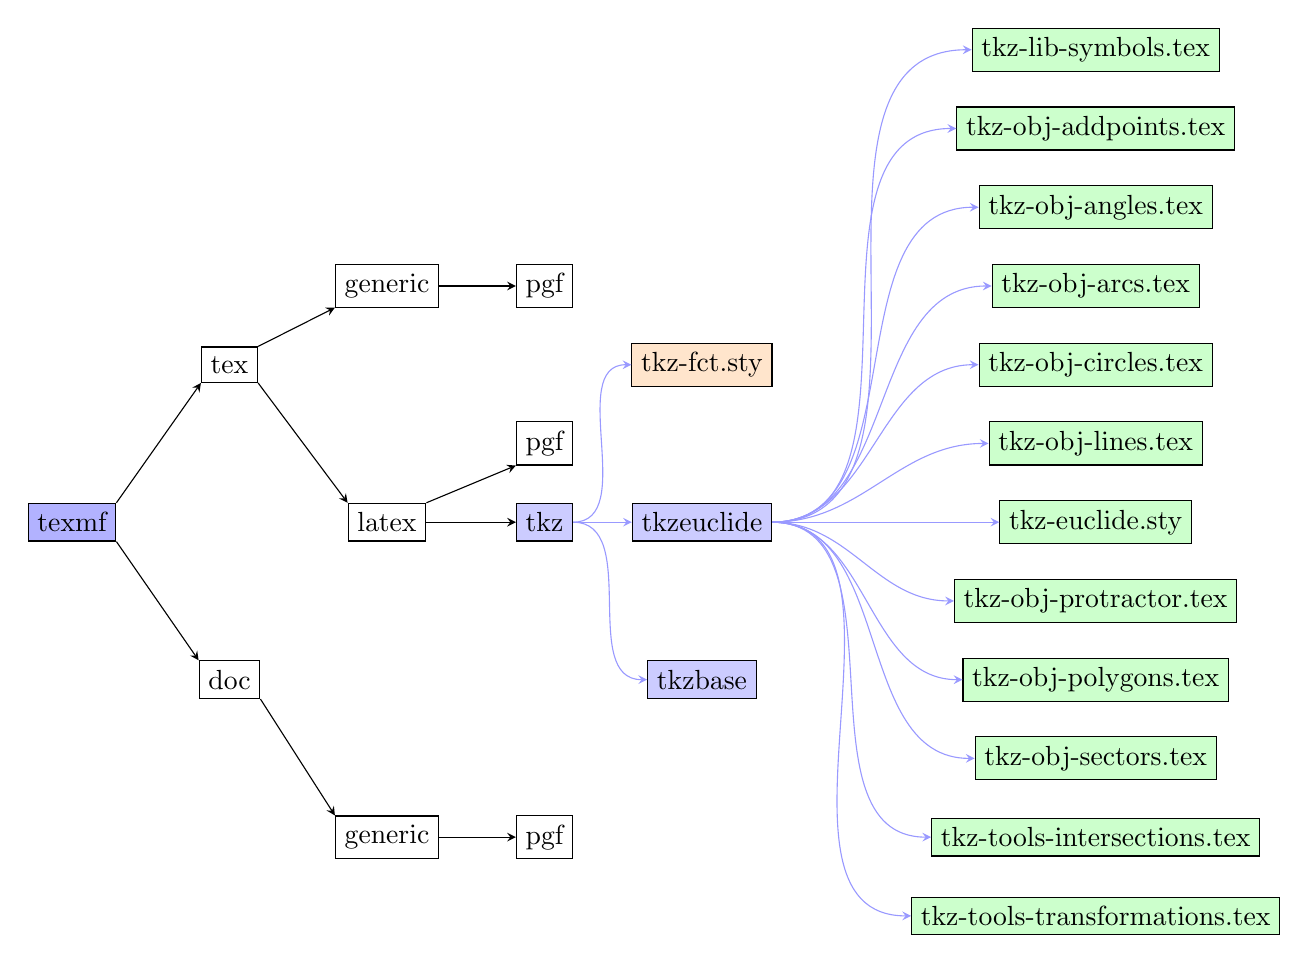
\begin{tikzpicture} [remember picture,rotate=90]

\node (texmf)   at (4,2)  [draw,fill=blue!30 ] {texmf};

\node (tex)     at (6,0)   [draw ] {tex};
\node (doc)     at (2,0)   [draw ] {doc};

\node (texgen)  at (7,-2)  [draw ] {generic};
\node (docgen)  at (0,-2)  [draw ] {generic};

\node (latex)   at (4,-2)  [draw ] {latex};

\node (genpgf)  at (7,-4)  [draw] {pgf};
\node (latpgf)  at (5,-4)  [draw] {pgf};
\node (tkz)     at (4,-4)  [draw,fill=blue!20 ] {tkz};

\node (docpgf)  at (0,-4)  [draw] {pgf};

\node (fct)     at (6,-6)  [draw,fill=orange!20] {tkz-fct.sty};
\node (tkb)     at (4,-6)  [draw,fill=blue!20] {tkzeuclide};
\node (tke)     at (2,-6)  [draw,fill=blue!20] {tkzbase};

\node (sym)     at (10,-11)  [draw,fill=green!20] {tkz-lib-symbols.tex};
\node (add)     at (9,-11)  [draw,fill=green!20] {tkz-obj-addpoints.tex};
\node (tuti)     at (8,-11)  [draw,fill=green!20] {tkz-obj-angles.tex};
\node (tmisc)    at (7,-11)  [draw,fill=green!20] {tkz-obj-arcs.tex};
\node (tmath)    at (6,-11)  [draw,fill=green!20] {tkz-obj-circles.tex};
\node (tbas)     at (5,-11)  [draw,fill=green!20] {tkz-obj-lines.tex};
\node (base)     at (4,-11)  [draw,fill=green!20] {tkz-euclide.sty};
\node (cfg)      at (3,-11)  [draw,fill=green!20]   {tkz-obj-protractor.tex};
\node (mark)     at (2,-11)  [draw,fill=green!20]   {tkz-obj-polygons.tex};
\node (pts)      at (1,-11)  [draw,fill=green!20]   {tkz-obj-sectors.tex};
\node (int) at (0,-11)  [draw,fill=green!20]   {tkz-tools-intersections.tex};
\node (tsf) at (-1,-11) [draw,fill=green!20]  {tkz-tools-transformations.tex};

\draw[-stealth](texmf.north east) --(tex.south west)    ;
\draw[-stealth](texmf.south east) -- (doc.north west)   ;

\draw[-stealth](tex.north east) --(texgen.south west)    ;
\draw[-stealth](tex.south east) -- (latex.north west)   ;
\draw[-stealth](texgen.east) -- (genpgf.west)   ;

\draw[-stealth](doc.south east) -- (docgen.north west)   ;
\draw[-stealth](docgen.east) -- (docpgf.west)   ;

\draw[-stealth](latex.north east) -- (latpgf.south west)   ;
\draw[-stealth](latex.east) -- (tkz.west)   ;

\draw[-stealth,blue!40](tkz.east) to[out=-90,in=90](fct.west) ;
\draw[-stealth,blue!40](tkz.east) to[out=-90,in=90](tkb.west) ;
\draw[-stealth,blue!40](tkz.east) to[out=-90,in=90](tke.west) ;

\draw[-stealth,blue!40](tkb.east) to[out=-90,in=90](sym.west) ;
\draw[-stealth,blue!40](tkb.east) to[out=-90,in=90](add.west) ;
\draw[-stealth,blue!40](tkb.east) to[out=-90,in=90](tuti.west) ;
\draw[-stealth,blue!40](tkb.east) to[out=-90,in=90](tmisc.west) ;
\draw[-stealth,blue!40](tkb.east) to[out=-90,in=90](tmath.west) ;
\draw[-stealth,blue!40](tkb.east) to[out=-90,in=90](tbas.west) ;
\draw[-stealth,blue!40](tkb.east) to[out=-90,in=90](base.west) ;
\draw[-stealth,blue!40](tkb.east) to[out=-90,in=90](cfg.west) ;
\draw[-stealth,blue!40](tkb.east) to[out=-90,in=90](mark.west) ;
\draw[-stealth,blue!40](tkb.east) to[out=-90,in=90](pts.west) ;
\draw[-stealth,blue!40](tkb.east) to[out=-90,in=90](int.west) ;
\draw[-stealth,blue!40](tkb.east) to[out=-90,in=90](tsf.west) ;

\end{tikzpicture}
\begin{tikzpicture}[remember picture,overlay]
        \path[-stealth,thin,red!40] (n1) edge [bend left] (tkz);
        \path[-stealth,thin,red!40] (n2) edge [bend left] (tkb);
\end{tikzpicture}
\begin{tcblisting}{}
\begin{tikzpicture}[scale=.8]
   \tkzInit[ymin=-1,ymax=6,xmin=-1,xmax=10]
   \tkzClip[space=.5] \tkzDefPoint(0,0){O}
   \tkzDefPoint(1,0){I} \tkzDefPoint(10,0){A}
   \tkzDefMidPoint(O,A) \tkzGetPoint{M}
   \tkzDefPointWith[orthogonal](I,M)
   \tkzGetPoint{H}   \tkzInterLC(I,H)(M,A)
   \tkzGetSecondPoint{B}  \tkzDrawSegment(O,A)
   \tkzDrawSegment[style=dashed](I,H)
\tkzDrawPoints(O,I,A,B,M)\tkzDrawArc(M,A)(O)
   \tkzMarkRightAngle(A,I,B)
   \tkzLabelSegment[right=4pt](I,B){$\sqrt{a}$}
   \tkzLabelSegment[below](O,I){$1$}
   \tkzLabelSegment[below](I,M){$a/2$}
   \tkzLabelSegment[below](M,A){$a/2$}
   \tkzLabelPoints(I,M,B,A)
   \tkzLabelPoint[below left](O){$O$}
\end{tikzpicture}
\end{tcblisting}
\begin{tcblisting}{sidebyside}
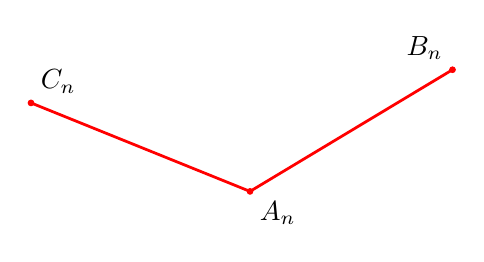
\begin{tikzpicture}
\tkzDefPoint[label=-60:$A_n$](2,3){A}
\tkzDefPoint[shift={(2,3)},%
label=above left:$B_n$](31:3){B}
\tkzDefPoint[shift={(2,3)},%
label=above right:$C_n$](158:3){C}
\tkzDrawSegments[color=red,%
line width=1pt](A,B A,C)
\tkzDrawPoints[color=red](A,B,C)
\end{tikzpicture}
\end{tcblisting}
\begin{tcblisting}{sidebyside}
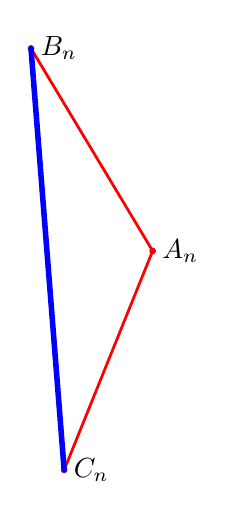
\begin{tikzpicture}[rotate=90]
\tkzDefPoint[label=right:$A_n$](2,3){A}
\begin{scope}[shift={(A)}]
\tkzDefPoint[label= right:$B_n$](31:3){B}
\tkzDefPoint[label= right:$C_n$](158:3){C}
\end{scope}
\tkzDrawSegments[color=red,%
line width=1pt](A,B A,C)
\tkzDrawPoints[color=red](A,B,C)
\tkzDrawSegments[blue,line width=2pt](C,B)
\end{tikzpicture}
\end{tcblisting}
\begin{tcblisting}{sidebyside}
\begin{tikzpicture}[scale=1]
\tkzInit[xmax=6,ymax=6]
\tkzGrid
\tkzSetUpPoint[shape = circle,color = red,%
size = 8,fill = red!30]
\tkzDefPoint(-1+1,-1+4){O}
\tkzDefPoint({3*ln(exp(1))},{exp(1)}){A}
\tkzDefPoint
({4*sin(FPpi/6)},{4*cos(FPpi/6)}){B}
\tkzDefPoint
({4*sin(FPpi/3)},{4*cos(FPpi/3)}){B'}
\tkzDefPoint(30:5){C}
\tkzDefPoint[shift={(1,3)}](45:4){A'}
\begin{scope}[shift=(A)]
\tkzDefPoint(30:3){C'}
\tkzDefPoint[label=left:$D$](-3,-2){D}
\end{scope}
\tkzDrawPoints[color=blue](O,B,C,D)
\tkzDrawPoints[color=red,%
shape=cross out](B',A,A',C')
\tkzLabelPoints(A,O,B,B',A',C,C')
\filldraw(0,2)coordinate(E)node[left]{$E$}circle(2pt);
\tkzDefMidPoint(A,B)\tkzGetPoint{F}
\fill(F)node[right]{F}circle(2pt);
\node(A)at({4*ln(exp(1))},{exp(1)}){G};
\end{tikzpicture}
\end{tcblisting}
\begin{tcblisting}{sidebyside}
\begin{tikzpicture}[scale=1]
\tkzSetUpLine[color=blue!60]
\begin{scope}[rotate=30]
\tkzDefPoint(2,3){A}
\begin{scope}[shift=(A)]
\tkzDefPoint(90:5){B}
\tkzDefPoint(30:5){C}
\end{scope}
\end{scope}
 \tkzDrawPolygon(A,B,C)
\tkzLabelPoints[above](B,C)
\tkzLabelPoints[below](A)
\end{tikzpicture}

\begin{tikzpicture}[rotate=30]
\draw[blue](2,3)coordinate(A)
node[black,below]{$A$}
--+(30:5)coordinate(C)
node[black,above]{$C$}
--++(90:5)coordinate(B)
node[black,above]{$B$}--(C)(B)--(A);
\end{tikzpicture}
\end{tcblisting}
\begin{tcblisting}{sidebyside}
\begin{tikzpicture}
\tkzSetUpPoint[size=3]
\tkzDefPoints{0/0/A,
2/0/B,%%坐标(2,2),点的名称为B
2/2/C,
0/2/D}
\tkzDrawSegments(D,A A,B B,C C,D)
\tkzDrawPoints(A,B,C,D)
\end{tikzpicture}
\end{tcblisting}
\begin{tcblisting}{sidebyside}
\begin{tikzpicture}
\tkzDefPoint(2,3){A}
\tkzDefShiftPoint[A](0:4){B}
\tkzDefShiftPoint[A](30:4){C}
\tkzDrawSegments(A,B B,C C,A)
\tkzMarkSegments[mark=oo,color=red](A,B A,C)
\tkzMarkSegments[mark=s|,color=red](B,C)
%%%标记线条功能
\tkzDrawPoints(A,B,C)
\tkzLabelPoints(B,C)
\tkzLabelPoints[above left](A)
\end{tikzpicture}
\end{tcblisting}
\begin{tcblisting}{sidebyside}
\begin{tikzpicture}[scale=.5]
\coordinate(A)at(2,3);
\coordinate(B)at(5,-1);
\tkzDefPoint[label=below:$\mathcal{C}$,
shift={(2,3)}](-30:5.5){E}
\draw(E)circle(2pt);
\begin{scope}[shift=(A)]
\tkzDefPoint(30:5){C}
\end{scope}
\tkzCalcLength[cm](A,B)
\tkzGetLength{rAB}
\tkzDrawCircle[R,dashed,draw=red](A,\rAB cm)
\tkzDrawCircle(B,A)
\tkzInterCC(A,B)(B,A)
\tkzGetPoints{F}{G}
\tkzLabelPoints(F,G)
\tkzDrawPoints(F,G)
\tkzDrawSegment(A,B)
\tkzDrawPoints(A,B,C)
\tkzLabelPoints(B,C)
\tkzLabelPoints[above](A)
\end{tikzpicture}
\end{tcblisting}
\begin{tcblisting}{sidebyside}
\begin{tikzpicture}
  \tkzDefPoint(0,0){A}
  \tkzDefPoint(4,0){B}
  \tkzDefPoint(0,3){C}
  \tkzDrawSegments(A,B B,C C,A)
  % \tkzDrawPolygon with
  % \usetkzobj{polygons}
  \tkzDrawPoints(A,B,C)
  \tkzLabelPoint[left,red](A){$A$}
  \tkzLabelPoint[right,blue](B){$B$}
  \tkzLabelPoint[above,purple](C){$C$}
\tkzMarkRightAngle[fill=red!20](C,A,B)%画直角
\end{tikzpicture}
\end{tcblisting}
\begin{tcblisting}{sidebyside}
\begin{tikzpicture}
\tkzDefPoint(2,3){A}
\tkzDefPoint(4,0){B}
\tkzDefMidPoint(A,B) \tkzGetPoint{C}
\tkzDrawSegment(A,B)
\tkzDrawPoints(A,B,C)
\tkzLabelPoints[right](A,B,C)
\end{tikzpicture}
\end{tcblisting}
\begin{tcblisting}{sidebyside}
\begin{tikzpicture}
\tkzDefPoint(2,3){A}
\tkzDefShiftPointCoord[2,3](30:4){B}
\tkzDefBarycentricPoint(A=1,B=2)
%%%画点组的质心
\tkzGetPoint{I}
\tkzDrawPoints(A,B,I)
\tkzDrawLine(A,B)
%%%带有0.2的前后延长,用add选项更改
%%例如\tkzDrawLine[add=0 and 0.3](A,B)
\tkzLabelPoints(A,B,I)
\end{tikzpicture}
\end{tcblisting}
\begin{tcblisting}{sidebyside}
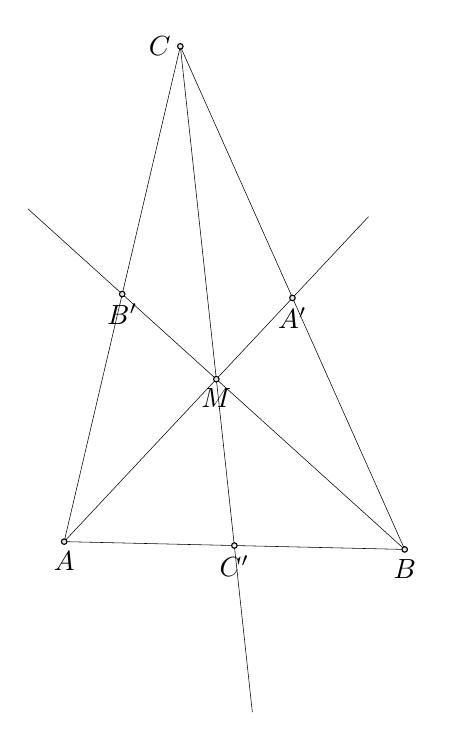
\begin{tikzpicture}[scale=1.2,rotate=-35]
\tkzInit[xmax=6,ymax=6]
\tkzDefPoint(2,1){A}
\tkzDefPoint(5,3){B}
\tkzDefPoint(0,6){C}
\tkzDrawPolygon(A,B,C)
\tkzDefBarycentricPoint(A=1,B=1,C=1)
%%%重心
\tkzGetPoint{M}
\tkzDrawLines[add=0 and 1](A,M B,M C,M)
\tkzDrawPoints(A,B,C,M)
\node[left]at(C){$C$};
\tkzLabelPoints(A,B,M)
\tkzDefMidPoint(A,B)  \tkzGetPoint{C'}
\tkzDefMidPoint(A,C)  \tkzGetPoint{B'}
\tkzDefMidPoint(C,B)  \tkzGetPoint{A'}
\tkzDrawPoints(A',B',C')
\tkzLabelPoints(A',B',C')
\end{tikzpicture}
\end{tcblisting}
\begin{tcblisting}{sidebyside}
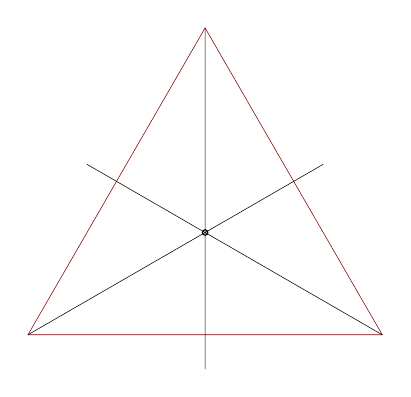
\begin{tikzpicture}[scale=.75]
\tkzDefPoint(-1,1){A}
\tkzDefPoint(5,1){B}
\tkzDefEquilateral(A,B)\tkzGetPoint{C}
\tkzDrawPolygon[color=Maroon](A,B,C)
\tkzCentroid(A,B,C)%%重心
\tkzGetPoint{G}
\tkzDrawPoint(G)
\tkzDrawLines[add = 0 and 2/3](A,G B,G C,G)
\end{tikzpicture}
\end{tcblisting}
\begin{tcblisting}{sidebyside}
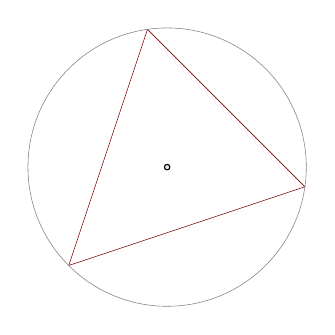
\begin{tikzpicture}
\tkzDefPoint(0,1){A}
\tkzDefPoint(3,2){B}
\tkzDefPoint(1,4){C}
\tkzDrawPolygon[color=Maroon](A,B,C)
\tkzCircumCenter(A,B,C)%%外心
\tkzGetPoint{G}
\tkzDrawPoint(G)
\tkzDrawCircle(G,A)
\end{tikzpicture}
\end{tcblisting}
\begin{tcblisting}{sidebyside}
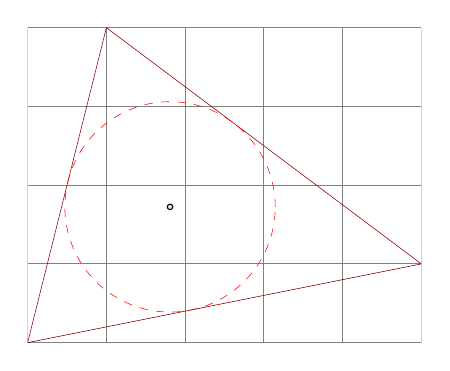
\begin{tikzpicture}
\tkzInit[xmax=5,ymax=4]
\tkzClip\tkzGrid
\tkzDefPoint(0,0){A}
\tkzDefPoint(5,1){B}
\tkzDefPoint(1,4){C}
\tkzDrawPolygon[color=Maroon](A,B,C)
\tkzInCenter(A,B,C)%%%内心
\tkzGetPoint{G}
\tkzDrawPoint(G)
%\tkzDrawLines[add = 0 and 2/3](A,G B,G C,G)
\tkzDefPointBy[projection=onto A--B](G)
\tkzGetPoint{D}
\tkzDrawCircle[dashed,color=red](G,D)
\end{tikzpicture}
\end{tcblisting}
\begin{tcblisting}{sidebyside}
\begin{tikzpicture}
%%矩形内,直线,线段和圆上取随机点
\tkzInit[xmax=5,ymax=5]  \tkzGrid
\tkzDefPoint(0,0){A}  \tkzDefPoint(2,2){B}
\tkzDefPoint(5,5){C}
\tkzGetRandPointOn[rectangle = A and B]{a}
\tkzGetRandPointOn[rectangle = B and C]{d}
\tkzDrawLine(a,d)
\tkzDrawPoints(A,B,C,a,d)
\tkzLabelPoints(A,B,C,a,d)
\tkzGetRandPointOn[segment=A--B]{D}
\tkzGetRandPointOn[line=B--C]{E}
\tkzCalcLength[cm](C,B)\tkzGetLength{rBC}
\tkzDrawCircle(C,B)
\tkzGetRandPointOn[circle=center C radius \rBC cm]{F}
\tkzLabelPoints(D,E,F)
\tkzDrawPoints(D,E,F)
\end{tikzpicture}
\end{tcblisting}
\begin{tcblisting}{sidebyside}
\begin{tikzpicture}[scale=.75]
\tkzDefPoint(0,0){A}
\tkzGetRandPointOn[circle= center A radius 4cm]{B}
\tkzDrawPoints(A,B)
\tkzDefPointBy[rotation= center A angle 180](B)
\tkzGetPoint{C}
\tkzInterCC[R](A,4 cm)(B,4 cm)
\tkzGetPoints{I}{I'}
\tkzInterCC[R](A,4 cm)(I,4 cm)
\tkzGetPoints{J}{B}
\tkzInterCC(B,A)(C,B)
\tkzGetPoints{D}{E}
\tkzInterCC(D,B)(E,B)
\tkzGetPoints{M}{M'}
\tikzset{arc/.style
={color=brown,style=dashed,delta=10}}
\tkzDrawArc[arc](C,D)(E)
\tkzDrawArc[arc,color=cyan](B,E)(D)
\tkzDrawCircle[color=blue,line width=.2pt](A,B)
\tkzDrawArc[arc](D,B)(M)
\tkzDrawArc[arc](E,M)(B)
\tkzCompasss[color=red,style=solid](B,I I,J J,C)
\tkzDrawPoints(B,C,D,E,M)
\tkzLabelPoints(A,B,C,D,E,M,I,I')
\end{tikzpicture}
\end{tcblisting}
\begin{tcblisting}{sidebyside}
\begin{tikzpicture}[scale=0.8]%%轴对称
\tkzInit[ymin=-4,ymax=6,xmin=-7,xmax=3]
\tkzClip
\tkzDefPoints{1.5/-1.5/C,-4.5/2/D}
\tkzDefPoint(-4,-2){O}
\tkzDefPoint(-2,-2){A}
\foreach \i in {0,1,...,4}{%
\pgfmathparse{0+\i * 72}
\tkzDefPointBy[rotation=center O angle \pgfmathresult](A) \tkzGetPoint{A\i}
\tkzDefPointBy[reflection = over C--D](A\i) \tkzGetPoint{A\i'}}
\tkzDrawPolygon(A0, A2, A4, A1, A3)
\tkzDrawPolygon(A0', A2', A4', A1', A3')
\tkzDrawLine[add= .5 and .5](C,D)
\tkzLabelPoints(O,A,C,D)
\tkzDrawPoints(O,A,C,D)
\end{tikzpicture}
\end{tcblisting}
\begin{tcblisting}{sidebyside}
\begin{tikzpicture}%%位似与投影
\tkzInit   \tkzClip
\tkzDefPoint(0,1){A}\tkzDefPoint(6,3){B}
\tkzDefPoint(3,6){C}
\tkzDrawLines[add= 0 and .3](A,B A,C)
\tkzDefLine[bisector](B,A,C)%角平分线
\tkzGetPoint{a}
\tkzDrawLine[add=0 and 0,color=magenta!50 ](A,a)
\tkzDefPointBy[homothety=center A ratio .5](a)   \tkzGetPoint{a'}
\tkzDefPointBy[projection = onto A--B](a')       \tkzGetPoint{k}
\tkzDrawSegment[style=dashed](a',k)
\tkzShowLine[bisector,size=2,gap=2](B,A,C)
\tkzDrawCircle(a',k)
\tkzDrawPoints(A,B,C,a,a',k)
\tkzLabelPoints(A,B,C,a,a',k)
\end{tikzpicture}
\end{tcblisting}
\begin{tcblisting}{sidebyside}
\begin{tikzpicture}[scale=1.2]
\tkzClip[space=1.5]
\tkzDefPoint(0,0){A}
\tkzDefPoint(0,4){B}
\tkzDrawTriangle[pythagore](B,A) \tkzGetPoint{C}
\tkzDefLine[bisector](B,C,A) \tkzGetPoint{c}
\tkzInterLL(C,c)(A,B)        \tkzGetPoint{D}
\tkzDrawSegment(C,D)
\tkzDrawCircle(D,A)
\tkzDefPointBy[projection=onto B--C](D) \tkzGetPoint{G}
\tkzInterLC(C,D)(D,A) \tkzGetPoints{E}{F}
\tkzDrawPoints(A,C,F) \tkzLabelPoints(A,C,F)
\tkzDrawPoints(B,D,E,G)
\tkzLabelPoints[above right](B,D,E,G)
\end{tikzpicture}
\end{tcblisting}
\begin{tcblisting}{sidebyside}
\begin{tikzpicture}%%对称
\tkzDefPoint(0,0){O}
\tkzDefPoint(2,-1){A}
\tkzDefPoint(2,2){B}
\tkzDefPointsBy[symmetry=center O](B,A){}
\tkzDrawLine(A,A')
\tkzDrawLine(B,B')
\tkzMarkAngle[mark=s,arc=lll,size=2 cm,mkcolor=red](A,O,B)
\tkzLabelAngle[pos=1,circle,draw,
fill=blue!10](A,O,B){$60^{\circ}$}
\tkzLabelPoints(O,A,B,A',B')
\end{tikzpicture}
\end{tcblisting}
\begin{tcblisting}{sidebyside}
\begin{tikzpicture}[scale=0.6,rotate=-90]
\tkzInit
\tkzPoint[pos=left](0,0){A} \tkzPoint(5,0){B}
\tkzDrawSegment(A,B)
\tkzDefPointBy[rotation= center A angle 60](B)
\tkzGetPoint{C}
\tkzDefPointBy[symmetry= center C](A)
\tkzGetPoint{D}
\tkzDrawSegment(A,tkzPointResult)
\tkzDrawLine(B,D)
\tkzDrawArc[delta=10](A,B)(C)
\tkzDrawArc[delta=10](B,C)(A)
\tkzDrawArc[delta=10](C,D)(D)
\tkzMarkRightAngle(D,B,A)
\tkzDrawPoints(D,C)
\tkzLabelPoints(D,C)
\end{tikzpicture}
\end{tcblisting}
\begin{tcblisting}{sidebyside}
\begin{tikzpicture}[scale=2]%反演
\tkzDefPoint(0,0){O}
\tkzDefPoint(1,0){A}
\tkzDrawCircle(O,A)
\tkzDefPoint(-1.5,-1.5){z1}
\tkzDefPoint(0.35,0){z2}
\tkzDrawPoints[fill=red,color=black,size=8](O,z1,z2)
\tkzDefPointBy[inversion = center O through A](z1)
\tkzGetPoint{Z1}
\tkzDefPointBy[inversion = center O through A](z2)
\tkzGetPoint{Z2}
\tkzDrawPoints[fill=red,color=black,size=8](Z1,Z2)
\tkzDrawSegments(z1,Z1 z2,Z2)
\tkzLabelPoints(O,A,z1,z2,Z1,Z2)
\end{tikzpicture}
\end{tcblisting}
\begin{tcblisting}{sidebyside}
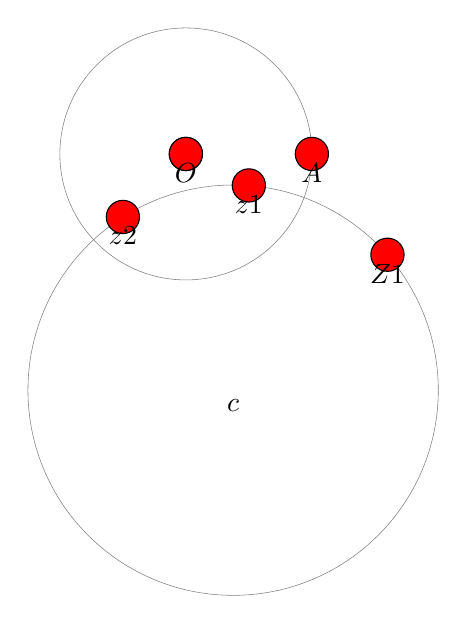
\begin{tikzpicture}[scale=1.6]
\tkzDefPoint(0,0){O}
\tkzDefPoint(1,0){A}
\tkzDrawCircle(O,A)
\tkzDefPoint(0.5,-0.25){z1}
\tkzDefPoint(-0.5,-0.5){z2}
\tkzDefPointBy[inversion = center O through A](z1)
\tkzGetPoint{Z1}
\tkzCircumCenter(z1,z2,Z1)\tkzGetPoint{c}
\tkzDrawCircle(c,Z1)
\tkzDrawPoints[color=black,
fill=red,size=12](O,z1,z2,Z1,O,A)
\tkzLabelPoints(O,A,z1,z2,Z1,c)
\end{tikzpicture}
\end{tcblisting}
\begin{tcblisting}{sidebyside}
\begin{tikzpicture}%%平移
\tkzDefPoint(0,0){A}  \tkzDefPoint(5,2){D}
\tkzDefPoint(3,0){B}  \tkzDefPoint(1,2){C}
\tkzDefPointsBy[translation= from A to D](B,C){E,F}
%%%如果这里的{E,F}写成{},则默认为{B',C'}
\tkzDrawPolygon[color=blue](A,B,C)
\tkzDrawPolygon[color=red](D,E,F)
\tkzDrawPoints[color=blue](A,B,C)
\tkzDrawPoints[color=red](D,E,F)
\tkzLabelPoints(A,B,D,E)
\tkzLabelPoints[above](C,F)
\tkzDrawSegments[color = gray,->,
style=dashed](A,D B,E C,F)
\end{tikzpicture}
\end{tcblisting}
\begin{tcblisting}{sidebyside}
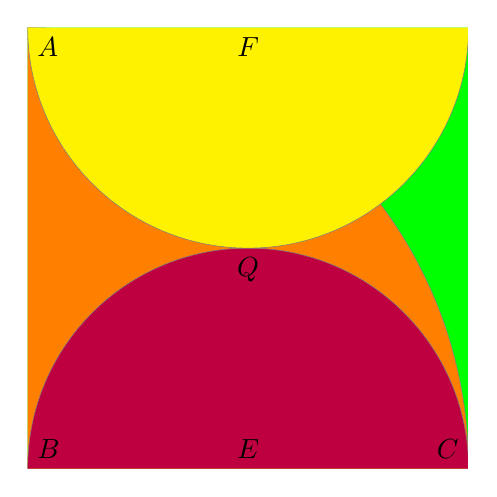
\begin{tikzpicture}[scale = 0.7]
\tkzDefPoint(0,0){B}
\tkzDefPoint(0,8){A}
\tkzDefSquare(A,B)
\tkzGetPoints{C}{D}
\tkzDrawSquare(A,B)
\tkzClipPolygon(A,B,C,D)
\tkzDefPoint(4,8){F}
\tkzDefPoint(4,0){E}
\tkzDefPoint(4,4){Q}
\tkzFillPolygon[color = green](A,B,C,D)
\tkzDrawCircle[fill   = orange](B,A)
\tkzDrawCircle[fill   = purple](E,B)
\tkzTgtFromP(F,A)(B)
\tkzInterLL(F,tkzFirstPointResult)(C,D)
\tkzInterLL(A,tkzPointResult)(F,E)
\tkzDrawCircle[fill = yellow](tkzPointResult,Q)
\tkzDefPointBy[projection= onto B--A](tkzPointResult)
\tkzDrawCircle[fill = blue!50!black](tkzPointResult,A)
\tkzLabelPoints(F,Q)\tkzLabelPoints[above right](B)
\tkzLabelPoints[below right](A)
\tkzLabelPoints[above](E)
\tkzLabelPoints[above left](C)
\end{tikzpicture}
\end{tcblisting}
\begin{tcblisting}{sidebyside}
\begin{tikzpicture}[scale=0.8]
\tkzInit[ymin=-3]
\tkzClip[space=1]
\tkzDefPoint(0,0){A}
\tkzDefPoint(8,0){B}
\tkzDefPoint(3.5,10){I}
\tkzDefMidPoint(A,B) \tkzGetPoint{O}
\tkzDefPointBy[projection=onto A--B](I) \tkzGetPoint{J}
\tkzInterLC(I,A)(O,A) \tkzGetPoints{M'}{M}
\tkzInterLC(I,B)(O,A)  \tkzGetPoints{N}{N'}
\tkzDrawCircle[diameter](A,B)
\tkzDrawSegments(I,A I,B A,B B,M A,N)
\tkzMarkRightAngles(A,M,B A,N,B)
\tkzDrawSegment[style=dashed,
color=blue](I,J)
\tkzShowTransformation[projection=onto A--B,color=red,size=3,gap=-3](I)
\tkzDrawPoints[color=red](M,N)
\tkzDrawPoints[color=blue](O,A,B,I)
\tkzLabelPoints(O)  \tkzLabelPoints[above right](N,I)
\tkzLabelPoints[below left](M,A)
\end{tikzpicture}
\end{tcblisting}
\begin{tcblisting}{sidebyside}
\begin{tikzpicture}[scale=0.75]
\tkzInit[xmin=0,xmax=8,ymin=-4,ymax=4]
\tkzDefPoint(0,0){A}  \tkzDefPoint(8,0){B}
\tkzDefMidPoint(A,B)  \tkzGetPoint{O}
\tkzDrawCircle(O,B)
\tkzDefMidPoint(O,B)  \tkzGetPoint{O'}
\tkzDrawCircle(O',B)
\tkzTangent[from=A](O',B) \tkzGetSecondPoint{E}
%%切线
\tkzInterLC(A,E)(O,B)     \tkzGetSecondPoint{D}
\tkzDefPointBy[projection=onto A--B](D)  \tkzGetPoint{F}
\tkzMarkRightAngle(D,F,B)
\tkzDrawSegments(A,D A,B D,F)
\tkzDrawSegments[color=red,line width=1pt,opacity=.4](A,O F,B)
\tkzDrawPoints(A,B,O,O',E,D)  \tkzLabelPoints(A,B,O,O',E,D)
\end{tikzpicture}
\end{tcblisting}
\begin{tcblisting}{sidebyside}
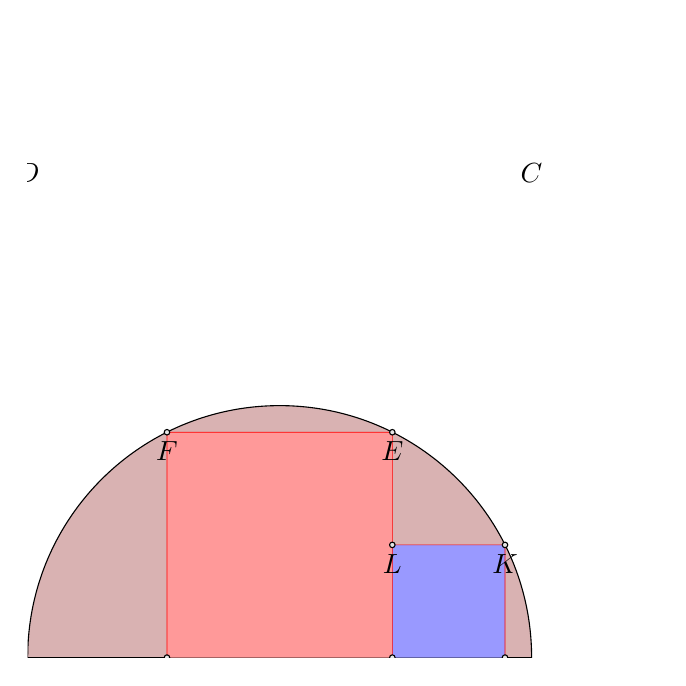
\begin{tikzpicture}[scale=0.8]
\tkzClip
\tkzDefPoint(0,0){A}
\tkzDefPoint(8,0){B}
\tkzDefPoint(4,0){I}
\tkzDefSquare(A,B)
\tkzGetPoints{C}{D}
\tkzInterLC(I,C)(I,B)
\tkzGetPoints{E'}{E}
\tkzInterLC(I,D)(I,B)
\tkzGetPoints{F'}{F}
\tkzDefPointsBy[projection =
onto A--B](E,F){H,G}
\tkzDefPointsBy[symmetry   = center H](I){J}
\tkzDefSquare(H,J)
\tkzGetPoints{K}{L}
\tkzDrawSector[fill=Maroon!30](I,B)(A)
\tkzFillPolygon[color=red!40](H,E,F,G)
\tkzFillPolygon[color=blue!40](H,J,K,L)
\tkzDrawPolySeg[color=red](H,E,F,G)
\tkzDrawPolySeg[color=red](J,K,L)
\tkzDrawPoints(E,G,H,F,J,K,L)
\tkzLabelPoints(A,B,C,D,E,F,G,H,I,J,K,L)
\end{tikzpicture}
\end{tcblisting}
\begin{tcblisting}{sidebyside}
\begin{tikzpicture}[scale=.8]
\tkzDefPoint(0,0){A} \tkzDefPoint(5,0){B}
\tkzDrawCircle[R,dashed](A,4 cm) \tkzDrawCircle[R,dashed](B,3 cm)
\tkzInterCC[R](A,4 cm)(B,3 cm) \tkzGetPoints{C}{D}
\tkzDrawPolygon(A,B,C)
\tkzCompasss(A,C B,C)
\tkzLabelSegment[below](A,B){$5$ cm}
\tkzLabelSegment[above left](A,C){$4$ cm}
\tkzLabelSegment[above right](B,C){$3$ cm}
\tkzDrawPoints[color=red](C)
\tkzDrawPoints[color=blue](A,B)
\end{tikzpicture}
\end{tcblisting}
\begin{tcblisting}{sidebyside}
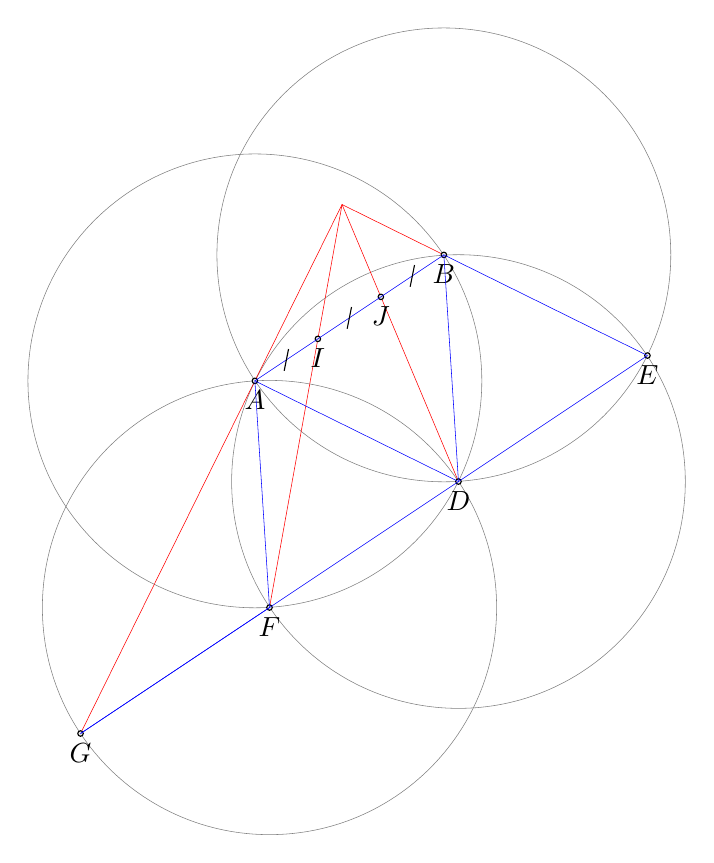
\begin{tikzpicture}[scale=.8]
\tkzDefPoint(0,0){A}  \tkzDefPoint(3,2){B}
\tkzInterCC(A,B)(B,A) \tkzGetPoints{C}{D}
\tkzInterCC(D,B)(B,A) \tkzGetPoints{A}{E}
\tkzInterCC(D,B)(A,B) \tkzGetPoints{F}{B}
\tkzInterLC(E,F)(F,A) \tkzGetPoints{D}{G}
\tkzInterLL(A,G)(B,E) \tkzGetPoint{O}
\tkzInterLL(O,D)(A,B) \tkzGetPoint{J}
\tkzInterLL(O,F)(A,B) \tkzGetPoint{I}
\tkzDrawCircle(D,A)    \tkzDrawCircle(A,B)
\tkzDrawCircle(B,A)    \tkzDrawCircle(F,A)
\tkzDrawSegments[color=red](O,G O,B O,D O,F)
\tkzDrawPoints(A,B,D,E,F,G,I,J)
\tkzLabelPoints(A,B,D,E,F,G,I,J)
\tkzDrawSegments[blue](A,B B,D A,D A,F F,G E,G B,E)
\tkzMarkSegments[mark=s|](A,I I,J J,B)
\end{tikzpicture}
\end{tcblisting}
\begin{tcblisting}{sidebyside}
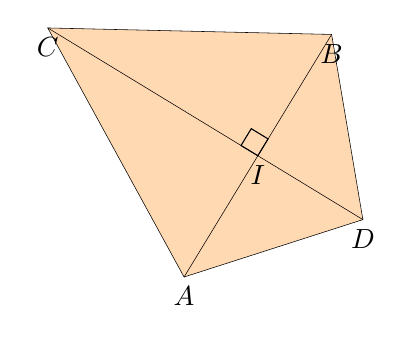
\begin{tikzpicture}[rotate=25]
\tkzInit
\tkzDefPoints{-2/0/A,1/2/B}
\tkzDefLine[mediator](A,B)%中垂线
\tkzGetPoints{C}{D}
\tkzDefPointWith[linear,K=.75](C,D)
\tkzGetPoint{D}
\tkzDefMidPoint(A,B)\tkzGetPoint{I}
\tkzFillPolygon[color=orange!30](A,C,B,D)
\tkzDrawSegments(A,B C,D)
\tkzMarkRightAngle(B,I,C)
\tkzDrawSegments(D,B D,A)
\tkzDrawSegments(C,B C,A)
\tkzLabelPoints(A,B,C,D,I)
\end{tikzpicture}
\end{tcblisting}
\begin{tcblisting}{sidebyside}
\begin{tikzpicture}
\tkzDefPoints{-1.5/-0.25/A,1/-0.75/B,-0.7/1/C}
\tkzDrawLine[end   = $(d_1)$](A,B)
\tkzDrawPoints(A,B,C)
\tkzDefLine[perpendicular=through C](B,A) \tkzGetPoint{c}
%%perpendicular可以换成orthogonal
\tkzDrawLine[end   = $(\delta)$](C,c)
\tkzInterLL(A,B)(C,c) \tkzGetPoint{I}
\tkzMarkRightAngle(C,I,B)
\tkzDefLine[parallel=through C](A,B) \tkzGetPoint{c'}
\tkzDrawLine[end   = $(d_2)$](C,c')
\tkzMarkRightAngle(I,C,c')
\tkzLabelPoints(A,B,C,c,c',C)
\end{tikzpicture}
\end{tcblisting}
\begin{tcblisting}{sidebyside}
\begin{tikzpicture}
\tkzInit[xmin=-3,xmax=6, ymin=-1,ymax=6]
\tkzClip
\tkzDefPoint(0,0){O}
\tkzDefPoint(3,1){I}
\tkzDefPoint(1,4){J}
\tkzDefLine[bisector](I,O,J)     \tkzGetPoint{i}
\tkzDefLine[bisector out](I,O,J) \tkzGetPoint{j}
\tkzDrawLines[add = 1 and 1,color=red](O,I O,J)
\tkzDrawLines[add = 5 and 5,color=blue](O,i O,j)
\tkzLabelPoints(O,I,J,i,j)
\end{tikzpicture}
\end{tcblisting}
\begin{tcblisting}{}
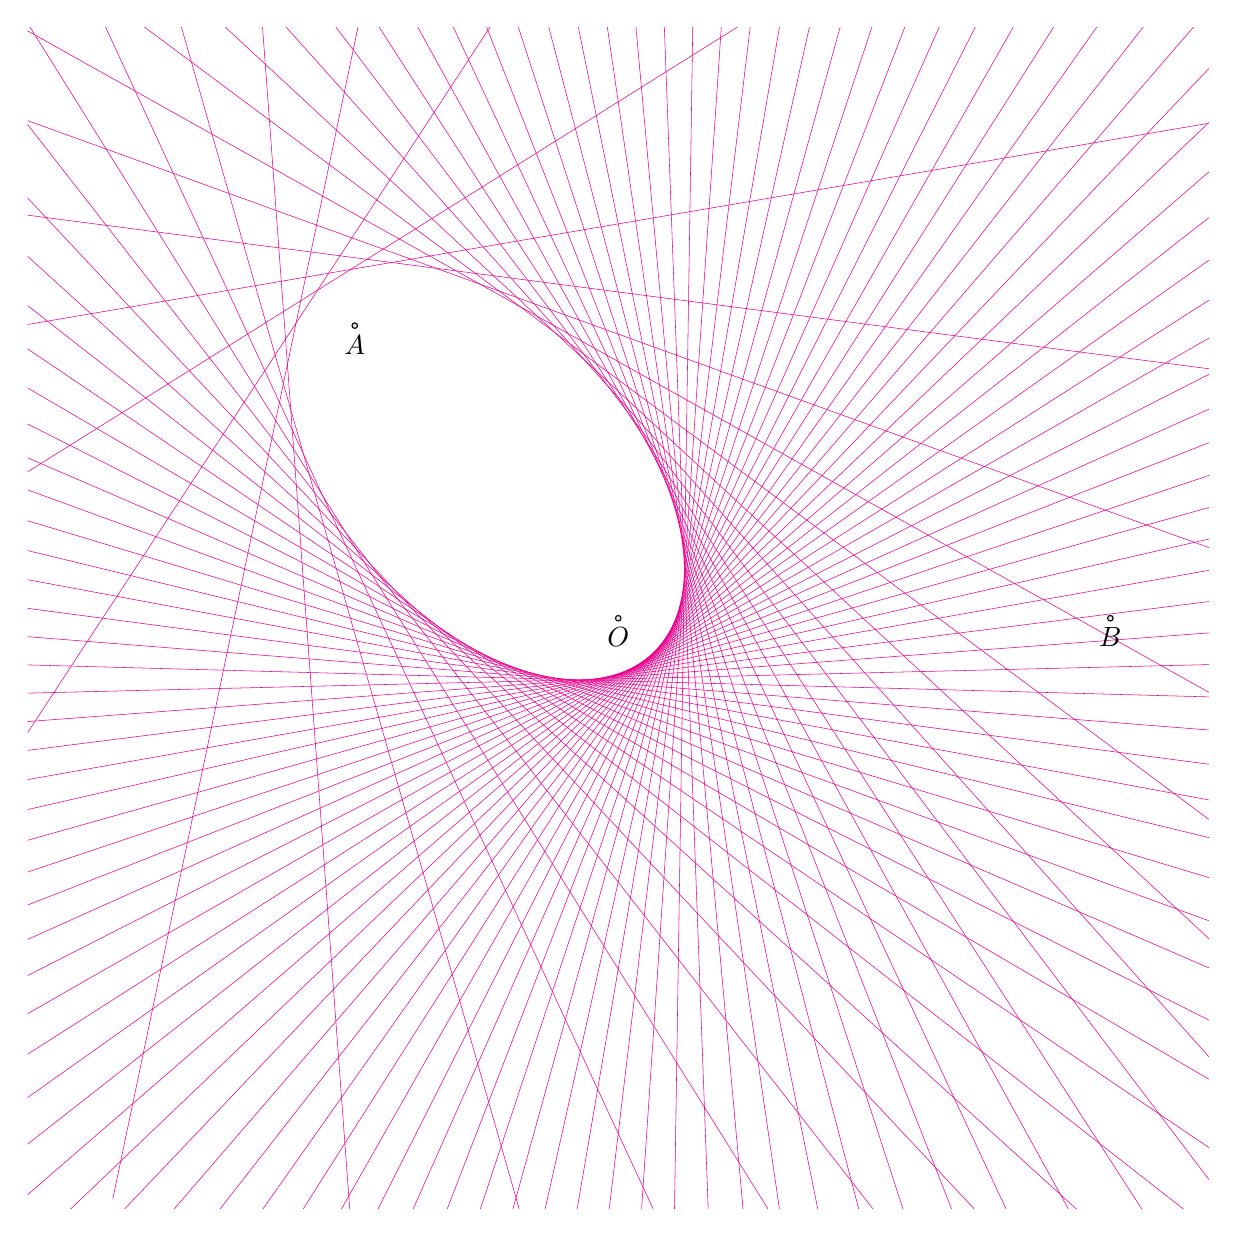
\begin{tikzpicture}[scale=1.25]
  \tkzInit[xmin=-6,ymin=-6,xmax=6,ymax=6]
  \tkzClip
  \tkzDefPoint(0,0){O}
  \tkzDefPoint(132:4){A}
  \tkzDefPoint(5,0){B}
  \foreach \ang in {5,10,...,360}{%
    \tkzDefPoint(\ang:5){M}
    \tkzDefLine[mediator](A,M)
    \tkzDrawLine[color=magenta,add= 4 and 4](tkzFirstPointResult,tkzSecondPointResult)}
  \tkzDrawPoints(O,A,B)\tkzLabelPoints(O,A,B)
  \end{tikzpicture}
\end{tcblisting}
\begin{tcblisting}{}
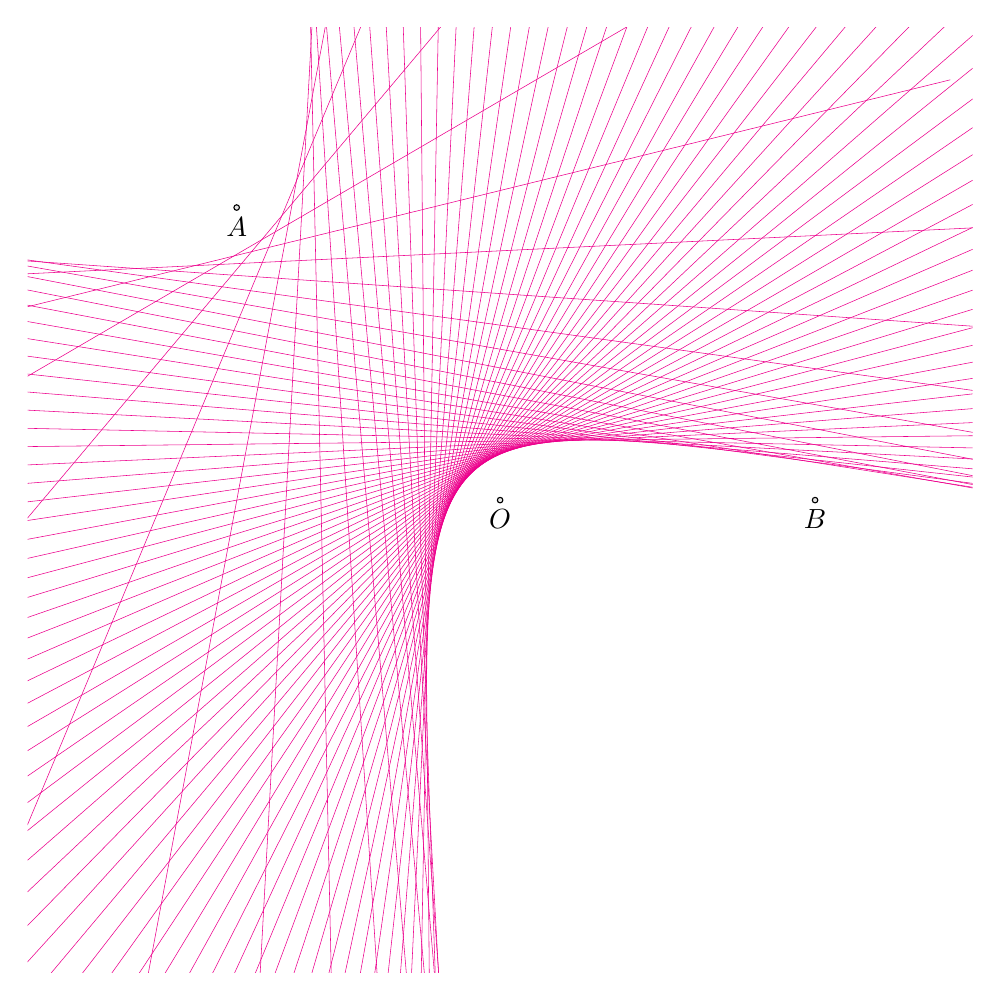
\begin{tikzpicture}
  \tkzInit[xmin=-6,ymin=-6,xmax=6,ymax=6]
  \tkzClip
  \tkzDefPoint(0,0){O}
  \tkzDefPoint(132:5){A}
  \tkzDefPoint(4,0){B}
  \foreach \ang in {5,10,...,360}{%
    \tkzDefPoint(\ang:4){M}
    \tkzDefLine[mediator](A,M)
    \tkzDrawLine[color=magenta,
             add= 4 and 4](tkzFirstPointResult,tkzSecondPointResult)}
  \tkzDrawPoints(O,A,B)\tkzLabelPoints(O,A,B)
   \end{tikzpicture}
\end{tcblisting}
\begin{tcblisting}{sidebyside}
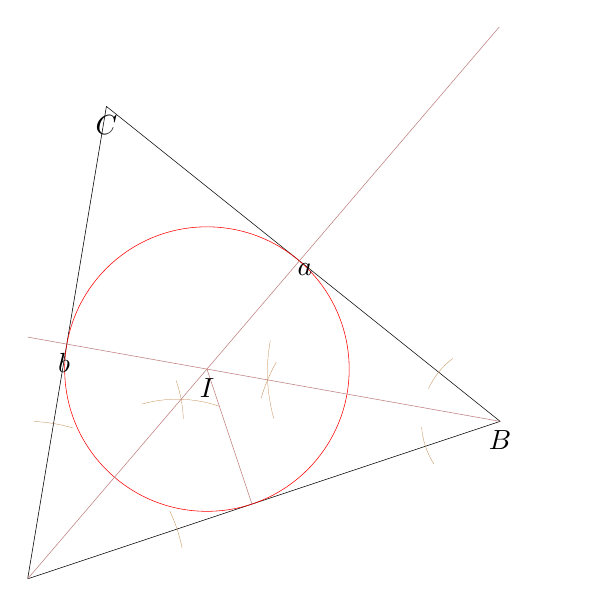
\begin{tikzpicture}
\tkzInit[xmin=0,xmax=7,ymin=0,ymax=7]
\tkzClip
\tkzDefPoints{0/0/A, 6/2/B, 1/6/C}
\tkzDrawPolygon(A,B,C)
\tkzSetUpCompass[color=brown,line width=.1 pt]
\tkzDefLine[bisector](B,A,C)  \tkzGetPoint{a}
\tkzDefLine[bisector](C,B,A)  \tkzGetPoint{b}
\tkzShowLine[bisector,size=2,gap=3](B,A,C)
\tkzShowLine[bisector,size=1,gap=3](C,B,A)
\tkzInterLL(A,a)(B,b) \tkzGetPoint{I}
\tkzDefPointBy[projection = onto A--B](I)
\tkzDrawCircle[radius,color=red,%
line width=.2pt](I,tkzPointResult)
\tkzDrawSegments[color=Maroon!50](I,tkzPointResult)
\tkzDrawLines[add=0 and 5,color=Maroon!50](A,a B,b)
\tkzLabelPoints(A,B,C,a,b,I)
\end{tikzpicture}
\end{tcblisting}
\begin{tcblisting}{sidebyside}
\begin{tikzpicture}
\tkzDefPoint(2,1){A}
\tkzDefPoint(6,4){B}
\tkzDrawSegment(A,B)
\tkzMarkSegment[color=Maroon,size=2pt,
        pos=0.4, mark=z](A,B)
\tkzMarkSegment[color=blue,
        pos=0.2, mark=oo](A,B)
\tkzMarkSegment[pos=0.8,
        mark=s,color=red](A,B)
\end{tikzpicture}
\end{tcblisting}
\begin{tcblisting}{sidebyside}
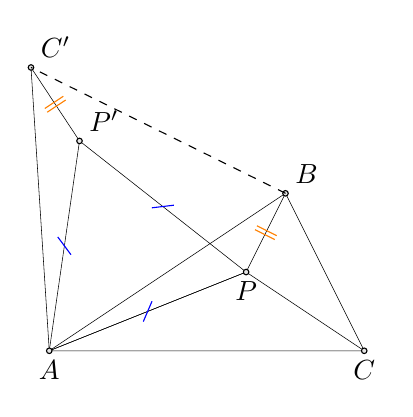
\begin{tikzpicture}
\tkzDefPoint(0,0){A}\tkzDefPoint(3,2){B}
\tkzDefPoint(4,0){C}\tkzDefPoint(2.5,1){P}
\tkzDrawPolygon(A,B,C)
\tkzDefEquilateral(A,P) \tkzGetPoint{P'}
\tkzDefPointsBy[rotation=center A angle 60](P,B){P',C'}
\tkzDrawPolygon(A,P,P')
\tkzDrawPolySeg(P',C',A,P,B)
\tkzDrawSegment(C,P)
\tkzDrawPoints(A,B,C,C',P,P')
\tkzMarkSegments[mark=s|,mark size=6pt,
color=blue](A,P P,P' P',A)
\tkzMarkSegments[mark=||,color=orange](B,P P',C')
\tkzLabelPoints(A,C) \tkzLabelPoints[below](P)
\tkzLabelPoints[above right](P',C',B)
\draw[dashed](B)--(C');
\end{tikzpicture}
\end{tcblisting}
\begin{tcblisting}{sidebyside}
\begin{tikzpicture}[scale=1.25]%%中线
\tkzDefPoint(0,0){A} \tkzDefPoint(4,0){B}
\tkzDefPoint(1,3){C} \tkzDrawPolygon(A,B,C)
\tkzSetUpLine[color=blue]
\tkzDrawMedian(A,B)(C)\tkzGetPoint{D}
\tkzDrawMedian(A,C)(B)\tkzGetPoint{E}
\tkzDrawMedian(B,C)(A)\tkzGetPoint{F}
\tkzLabelPoints(A,B,C,D,E,F)
\end{tikzpicture}
\end{tcblisting}
\begin{tcblisting}{sidebyside}
\begin{tikzpicture}[scale=1.25]
\tkzDefPoint(0,0){A} \tkzDefPoint(4,0){B}
\tkzDefPoint(1,3){C} \tkzDrawPolygon(A,B,C)
\tkzSetUpLine[color=magenta]
\tkzDrawAltitude(A,B)(C)\tkzGetPoint{D}
\tkzDrawAltitude(A,C)(B)\tkzGetPoint{E}
\tkzDrawAltitude(B,C)(A)\tkzGetPoint{F}
\tkzInterLL(C,D)(B,E)\tkzGetPoint{H}
\tkzLabelPoints(A,B,C,D,E,F,H)
\end{tikzpicture}
\end{tcblisting}
\begin{tcblisting}{sidebyside}
\begin{tikzpicture}
\tkzInit[xmin=-1,xmax=5,ymin=-1,ymax=4] \tkzClip
\tkzDefPoint(0,0){A} \tkzDefPoint(4,0){B}
\tkzDefPoint(1,3){C} \tkzDrawPolygon(A,B,C)
\tkzSetUpLine[color=purple]
\tkzDrawBisector(C,B,A)
\tkzDrawBisector(B,A,C)
\tkzDrawBisector(A,C,B)
\tkzLabelPoints(A,B,C)
\end{tikzpicture}
\end{tcblisting}
\begin{tcblisting}{sidebyside}
\begin{tikzpicture}[scale=1.5]
\tkzInit[xmin=0,xmax=4,ymin=0,ymax=2]
\tkzClip[space=.5]   \tkzDefPoint(0,0){A}
\tkzDefPoint(3,0){B} \tkzDefPoint(4,2){C}
\tkzDefPointWith[colinear= at C](B,A)
\tkzGetPoint{D}
\tkzDrawPolygon(A,B,C,D)
\tkzLabelPoints(A,B)
\tkzLabelPoints[above right](C,D)
\end{tikzpicture}
\end{tcblisting}
\begin{tcblisting}{sidebyside}
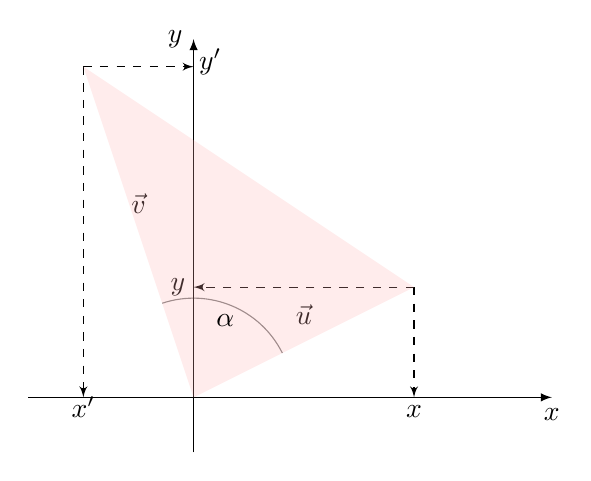
\begin{tikzpicture}[scale=0.7]
\tkzInit[xmin=-3,xmax=6,ymin=-1,ymax=6]
\tkzDrawX[noticks]
\tkzDrawY[noticks]
\tkzDefPoint(0,0){O}  \tkzDefPoint(4,2){A}
\tkzDefPoint(-2,6){B}
\tkzPointShowCoord[xlabel=$x$,ylabel=$y$](A)
%%显示点的坐标
\tkzPointShowCoord[xlabel=$x'$,ylabel=$y'$,%
                   ystyle={right=2pt}](B)
\tkzDrawVectors(O,A O,B)
\tkzLabelSegment[above=3pt](O,A){$\vec{u}$}
\tkzLabelSegment[above=3pt](O,B){$\vec{v}$}
\tkzMarkAngle[fill= yellow,size=1.8cm,%
              opacity=.5](A,O,B)
\tkzFillPolygon[red!30,opacity=0.25](A,B,O)
\tkzLabelAngle[pos = 1.5](A,O,B){$\alpha$}
\end{tikzpicture}
\end{tcblisting}
\begin{tcblisting}{sidebyside}
\begin{tikzpicture}
\tkzDefPoint(0,4){A}
\tkzDefPoint(3,2){B}
\tkzDefCircle[radius](A,B)
\tkzGetLength{rABpt}
\tkzpttocm(\rABpt){rABcm}
\tkzDrawCircle(A,B)
\tkzDrawPoints(A,B)
\tkzLabelPoints(A,B)
\tkzLabelCircle[draw,fill=Gold,%
text width=3cm,text centered](A,B)(-90)%
{La mesure du rayon est :
\rABpt pt soit \rABcm cm}
\end{tikzpicture}
\end{tcblisting}
\begin{tcblisting}{sidebyside}
\begin{tikzpicture}
\tkzInit[xmin=0,xmax=6,ymin=-3,ymax=3]
\tkzClip
\tkzDefPoint(2,2){A}
\tkzDefPoint(5,-2){B}
\tkzDefPoint(1,-2){C}
\tkzDefCircle[in](A,B,C)
\tkzGetPoint{I}    \tkzGetLength{rIN}
\tkzDefCircle[circum](A,B,C)
\tkzGetPoint{K}   \tkzGetLength{rCI}
\tkzDrawPoints(A,B,C,I,K)
\tkzDrawCircle[R,color=blue](I,\rIN pt)
\tkzDrawCircle[R,color=red](K,\rCI pt)
\tkzLabelPoints[below](B,C)
\tkzLabelPoints[above left](A,I,K)
\tkzDrawPolygon(A,B,C)
\end{tikzpicture}
\end{tcblisting}
\begin{tcblisting}{sidebyside}
\begin{tikzpicture}
\tkzDefPoint(0,0){A}
\tkzDefPoint(4,0){B}
\tkzDefCircle[apollonius,K=2](A,B)
\tkzGetPoint{K1}%%阿氏圆
\tkzGetLength{rAp}
\tkzDrawCircle[R,color = blue!50!black,
fill=blue!20,opacity=.4](K1,\rAp pt)
\tkzDefCircle[apollonius,K=3](A,B)
\tkzGetPoint{K2}   \tkzGetLength{rAp}
\tkzDrawCircle[R,color=red!50!black,
fill=red!20,opacity=.4](K2,\rAp pt)
\tkzLabelPoints[below](A,B,K1,K2)
\tkzDrawPoints(A,B,K1,K2)
\tkzDrawLine[add=.2 and 1](A,B)
\end{tikzpicture}
\end{tcblisting}
\begin{tcblisting}{sidebyside}
\begin{tikzpicture}
\tkzInit[xmin=-1,ymin=-1,xmax=8,ymax=6] \tkzClip
\tkzDefPoint(5,3.5){A} \tkzDefPoint(0,0){B} \tkzDefPoint(7,0){C}
\tkzDefCircle[euler](A,B,C)
\tkzGetPoint{E}  \tkzGetLength{rEuler}
%%九点圆
\tkzDrawPoints(A,B,C,E)
\tkzDrawCircle[R,blue](E,\rEuler pt)
\tkzDrawPolygon(A,B,C)
\tkzLabelPoints[below](B,C)  \tkzLabelPoints[left](A,E)
\end{tikzpicture}
\end{tcblisting}
\begin{tcblisting}{sidebyside}
\begin{tikzpicture}[scale=0.8]
\tkzDefPoint(0,0){O}  \tkzDefPoint(1,0){A}
\tkzDefPoint(1.5,1.25){B}  \tkzDefPoint(-2,-3){C}
\tkzDrawCircle(O,A)
\tkzDefCircle[orthogonal from=B](O,A)%%正交圆圆心
\tkzDrawCircle[thick,color=red](B,tkzFirstPointResult)
\tkzDefCircle[orthogonal from=C](O,A)
\tkzDrawCircle[thick,color=red](C,tkzFirstPointResult)
\tkzDrawPoints(tkzFirstPointResult,tkzSecondPointResult,O,A,B,C)
\tkzLabelPoints(O,A,C,B)
\end{tikzpicture}
\end{tcblisting}
\begin{tcblisting}{sidebyside}
\begin{tikzpicture}[scale=1.8]
\tkzDefPoint(0,0){O}
\tkzDefPoint(1,0){A}
\tkzDrawCircle(O,A)
\tkzDefPoint(-1.5,-1.5){z1}
\tkzDefPoint(1.5,-1.25){z2}
\tkzDefCircle[orthogonal through=
z1 and z2](O,A) \tkzGetPoint{c}%%正交圆切点
\tkzDrawCircle[thick,color=red](tkzPointResult,z1)
\tkzDrawPoints[fill=red,color=black,size=4](O,A,z1,z2,c)
\tkzLabelPoints(O,A,z1,z2,c)
\end{tikzpicture}
\end{tcblisting}
\begin{tcblisting}{sidebyside}
\begin{tikzpicture}
\tkzDefPoint(0,0){O}
\tkzDefPoint(3,0){A}
\tkzDrawCircle[color=blue,style=dashed](O,A)
\tkzDrawCircle[diameter,color=red,%
line width=2pt,fill=red!40,%
opacity=.5](O,A)
\tkzDrawCircle[R,color=orange](O,2.72 cm)
\end{tikzpicture}
\end{tcblisting}
\begin{tcblisting}{sidebyside}
\begin{tikzpicture}[scale=0.8]
\tkzDefPoint(0,0){O}
\tkzDefPoint(2,0){A}
\foreach \ang in {5,10,...,360}{%
\tkzDefPoint(\ang:2){M}
\tkzDrawCircle(M,A)
}
\end{tikzpicture}
\end{tcblisting}
\begin{tcblisting}{sidebyside}
\begin{tikzpicture}[scale=.333]
\tkzInit[xmin=-10,xmax=10,ymin=-10,ymax=10]
\tkzDefPoint(0 , 0){O}\tkzDefPoint(9 , 0){A}
\tkzDefPoint(-9, 0){C}\tkzDefPoint(0 , 9){B}
\tkzDefPoint(0 ,-9){D} \tkzClipCircle(O,A)
\foreach \pti in {1,2,...,8}{
\tkzDefPoint(10*\pti:9){P\pti}
\tkzDefPoint(90:\pti){MP\pti}
\tkzDefPoint(0: \pti){NP\pti}
\tkzDefLine[mediator](MP\pti,P\pti)
\tkzInterLL(B,D)(tkzFirstPointResult,tkzSecondPointResult)
\tkzDrawCircle[color=Maroon](tkzPointResult,P\pti)
}
\foreach \pti in {-1,-2,...,-8}{
\tkzDefPoint(10*\pti:9){P\pti}
\tkzDefPoint(-90:-\pti){MP\pti}
\tkzDefPoint(0: -\pti){NP\pti}
\tkzDefLine[mediator](MP\pti,P\pti)
\tkzInterLL(B,D)(tkzFirstPointResult,tkzSecondPointResult)
\tkzDrawCircle[color=Maroon](tkzPointResult,P\pti)
}
\foreach \pti in {1,2,...,8}{
\tkzDefLine[mediator](B,NP\pti)
\tkzInterLL(A,C)(tkzFirstPointResult,tkzSecondPointResult)
\tkzDrawCircle[color=Maroon](tkzPointResult,NP\pti)
}
\foreach \pti in {1,2,...,8}{
\tkzDefPoint(0: -\pti){NP\pti}
\tkzDefLine[mediator](B,NP\pti)
\tkzInterLL(A,C)(tkzFirstPointResult,tkzSecondPointResult)
\tkzDrawCircle[color=Maroon](tkzPointResult,NP\pti)
}
\tkzDrawCircle[R,color=Maroon](O,9 cm)
\tkzDrawSegments[color=Maroon](A,C B,D)
\end{tikzpicture}
\end{tcblisting}
\begin{tcblisting}{sidebyside}
\begin{tikzpicture}[scale=.5]
\tkzInit\tkzDefPoint(0,0){O}
\tkzDefPoint(6,6){E}
\tkzGetRandPointOn[circle=center O radius 4cm]{A}
\tkzDrawSegment(O,A)\tkzDrawCircle(O,A)
\tkzTangent[at=A](O)\tkzGetPoint{h}
\tkzTangent[from=E](O,A)\tkzGetPoints{e}{f}
\tkzTangent[from with R=E](O,3 cm)
\tkzGetPoints{k}{l}
\tkzDrawLine[add = 5 and 4](A,h)
\tkzMarkRightAngle[fill=red!30](O,A,h)
\tkzDrawLines[](E,e E,l)
\tkzDrawCircle(O,l)
\tkzLabelPoints(O,A,h,e,f,E,k,l)
\end{tikzpicture}
\end{tcblisting}
\begin{tcblisting}{sidebyside}
\begin{tikzpicture}[scale=0.75]
\tkzDefPoint(3,3){c}
\tkzDefPoint(6,3){a0}
\tkzRadius=1 cm
\tkzDrawCircle[R](c,\tkzRadius)
\foreach \an in {0,10,...,350}{
\tkzDefPointBy[rotation=center c angle \an](a0)
\tkzGetPoint{a}
\tkzTangent[from with R = a](c,\tkzRadius)
\tkzGetPoints{e}{f}
\tkzDrawLines[color=magenta](a,f a,e)
\tkzDrawSegments(c,e c,f)}
\end{tikzpicture}
\end{tcblisting}
\begin{tcblisting}{sidebyside}
\begin{tikzpicture}[scale=0.6]
\tkzInit[xmin=-4.1,xmax=5.2,ymin=-4.1,ymax=8]
\tkzClip[space=.5]
\tkzDefPoint(100:8){A}\tkzDefPoint(50:8){B}
\tkzDefPoint(0,0){C} \tkzDefPoint(0,4){R}
\tkzDrawCircle(C,R)
\tkzTangent[from = A](C,R)  \tkzGetPoints{D}{E}
\tkzTangent[from = B](C,R)  \tkzGetPoints{F}{G}
\tkzDrawSector[fill=blue!80!black,opacity=0.5](A,D)(E)
\tkzFillSector[color=red!80!black,opacity=0.5](B,F)(G)
\tkzInterCC(A,D)(B,F) \tkzGetSecondPoint{I}
\tkzDrawPoint[color=black](I)
\end{tikzpicture}
\end{tcblisting}
\begin{tcblisting}{sidebyside}
\begin{tikzpicture}[scale=1]
\tkzDefPoint(0,0){O}
\tkzDefPoint(-30:3){A}
\tkzDefPointBy[rotation = center O angle -60](A)
\tkzDrawSector[fill=red!50](O,A)(tkzPointResult)
\begin{scope}[shift={(-60:1cm)}]
\tkzDefPoint(0,0){O}
\tkzDefPoint(-30:3){A}
\tkzDefPointBy[rotation = center O angle -60](A)
\tkzDrawSector[fill=blue!50](O,tkzPointResult)(A)
\end{scope}
\end{tikzpicture}
\end{tcblisting}
\begin{tcblisting}{sidebyside}
\begin{tikzpicture}[scale=.5]
\tkzDefPoint(2,3){A}
\tkzDefPoint[shift={(2,3)}](31:8){B}
\tkzDefPoint[shift={(2,3)}](158:8){C}
\tkzDrawSegments[color = red,
           line width = 1pt](A,B A,C)
\tkzProtractor[with  = full,
               scale = 1.25](A,B)
\end{tikzpicture}
\end{tcblisting}
\begin{tcblisting}{sidebyside}
\begin{tikzpicture}[scale=.5]
\tkzInit[xmin=-4,xmax=9,ymin=-3,ymax=9]
\tkzClip  \tkzDefPoint(2,3){A}
\tkzDefPoint[shift={(2,3)}](31:8){B}
\tkzDefPoint[shift={(2,3)}](158:8){C}
\tkzDrawSegments[color=red,line width=1pt](A,B A,C)
\tkzProtractor[scale=1.25,with=full,return](A,C)
\end{tikzpicture}
\end{tcblisting}
\begin{tcblisting}{}
\begin{tikzpicture}
  \tkzInit
  \tkzDefPoint(1,5){A} \tkzDefPoint(5,2){B}  \tkzDrawSegment(A,B)
  \tkzFindSlopeAngle(A,B)\tkzGetAngle{tkzang}
  \tkzDefPointBy[rotation= center A angle \tkzang ](B) \tkzGetPoint{C}
  \tkzDefPointBy[rotation= center A angle -\tkzang ](B) \tkzGetPoint{D}
  \tkzCompass[length=1,dashed,color=red](A,C)
  \tkzCompass[delta=10,Maroon](B,C)   \tkzDrawPoints(A,B,C,D)
  \tkzLabelPoints(B,C,D)  \tkzLabelPoints[above left](A)
  \tkzDrawSegments[style=dashed](A,C A,D)
\end{tikzpicture}
\end{tcblisting}
\begin{tcblisting}{}
\begin{tikzpicture}[scale=.8,rotate=60]
  \tkzDefPoint(6,0){X}   \tkzDefPoint(3,3){Y}
  \tkzDefShiftPoint[X](-110:6){A}    \tkzDefShiftPoint[X](-70:6){B}
  \tkzDefShiftPoint[Y](-110:4.2){A'} \tkzDefShiftPoint[Y](-70:4.2){B'}
  \tkzDefPointBy[translation= from A' to B ](Y) \tkzGetPoint{Y}
  \tkzDefPointBy[translation= from A' to B ](B') \tkzGetPoint{C}
  \tkzInterLL(A,B)(X,Y) \tkzGetPoint{O}
  \tkzDefMidPoint(X,Y) \tkzGetPoint{I}
  \tkzDefPointWith[orthogonal](I,Y)
  \tkzInterLL(I,tkzPointResult)(A,B) \tkzGetPoint{Z}
  \tkzDrawCircle[circum](X,Y,B)
  \tkzDrawLines[add = 0 and 1.5](A,C) \tkzDrawLines[add = 0 and 3](X,Y)
  \tkzDrawSegments(A,X B,X B,Y C,Y)   \tkzDrawSegments[color=red](X,Z Y,Z)
  \tkzDrawPoints(A,B,C,X,Y,O,Z)
  \tkzLabelPoints(A,B,C,Z)   \tkzLabelPoints[above right](X,Y,O)
\end{tikzpicture}
\end{tcblisting}
\begin{tcblisting}{}
\begin{tikzpicture}[scale=1.25]
  \tkzDefPoint(0,0){A}
  \tkzDefPoint(3,0){B}
  \tkzDefPoint(9,0){C}
  \tkzDefPoint(1.5,2){X}
  \tkzDefPoint(6,4){Y}
   \tkzDefCircle[circum](X,Y,B) \tkzGetPoint{O}
  \tkzDefMidPoint(X,Y)               \tkzGetPoint{I}
  \tkzDefPointWith[orthogonal](I,Y)  \tkzGetPoint{i}
  \tkzDrawLines[add = 2 and 1,color=orange](I,i)
  \tkzInterLL(I,i)(A,B)              \tkzGetPoint{Z}
  \tkzInterLC(I,i)(O,B)              \tkzGetSecondPoint{M}
    \tkzDefPointWith[orthogonal](B,Z)  \tkzGetPoint{b}
  \tkzDrawCircle(O,B)
  \tkzDrawLines[add = 0 and 2,color=orange](B,b)
   \tkzDrawSegments(A,X B,X B,Y C,Y A,C X,Y)
   \tkzDrawSegments[color=red](X,Z Y,Z)
  \tkzDrawPoints(A,B,C,X,Y,Z,M,I)
   \tkzLabelPoints(A,B,C,Z)
   \tkzLabelPoints[above right](X,Y,M,I)
\end{tikzpicture}
\end{tcblisting}
\begin{tcblisting}{}
\begin{tikzpicture}[scale=1.25]
  \tkzInit[xmin= 0,xmax=8 ,ymin=0 ,ymax=7 ] \tkzClip[space=.5]
   \tkzDefPoint(0,0){C}
   \tkzDefPoint(7,0){B}
   \tkzDefPoint(5,6){A}
   \tkzDrawPolygon(A,B,C)
   \tkzDefMidPoint(C,B)          \tkzGetPoint{I}
   \tkzDrawArc(I,B)(C)
   \tkzInterLC(A,C)(I,B)        \tkzGetSecondPoint{B'}
   \tkzInterLC(A,B)(I,B)        \tkzGetFirstPoint{C'}
   \tkzInterLL(B,B')(C,C')      \tkzGetPoint{H}
   \tkzInterLL(A,H)(C,B)        \tkzGetPoint{A'}
   \tkzDrawCircle[circum,color=red](A,B',C')
   \tkzDrawSegments[color=orange](B,B' C,C' A,A')
   \tkzMarkRightAngles(C,B',B B,C',C C,A',A)
   \tkzDrawPoints(A,B,C,A',B',C',H)
   \tkzLabelPoints(A,B,C,A',B',C',H)
\end{tikzpicture}
\end{tcblisting}
\end{document} 